\documentclass[exercice]{thedocument}%
\startdatakeys
\source{}
\BO{2026}
\cycle{4}
\competencesDuSocle{RE}
\objectifsApprentissage{B2db,B1eb,B1ei}
\automatismes{B1cb,B2bb}
\enddatakeys
\begin{document}%
Sur la figure suivante les triangles ABC et A'B'C' sont symétriques par
    rapport à la droite (d).\par\bigskip
    {\centering
    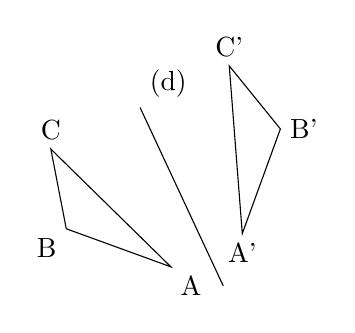
\begin{tikzpicture}[rotate=25,scale=0.5]
        \draw(0,0)--(0,5);
        \draw node[above right] at(0,5){(d)};
        \coordinate[label=below right:A](A)at(-1,1);
        \coordinate[label=below left:B](B)at(-3,3);
        \coordinate[label=C](C)at(-2.5,5);
        \coordinate[label=below:A'](A')at(1,1);
        \coordinate[label=right:B'](B')at(3,3);
        \coordinate[label=C'](C')at(2.5,5);
        \draw(A)--(B)--(C)--cycle;
        \draw(A')--(B')--(C')--cycle;
    \end{tikzpicture}
    \par}\medskip
    Quels angles sont égaux sur la figure ci dessus~?
\end{document}
